\section{Introduction}
Engineering, biological and knowledge graphs are checked against requirement patterns. A pattern graph names \emph{roles} (a pump, a supporting beam, a protein with a given function), and the check asks whether the entities that play those roles in an observed graph carry the expected observations. A natural implementation finds one embedding of the pattern with a subgraph matcher and reads the observations at the matched entities. This is correct only when the embedding is unique, and it often is not: in the third-party HPRD query workload that IdCon uses, \hprdAutoOrbitMulti{} of \hprdCountFullQueries{} queries have more than one embedding even when every query vertex must match its own protein label and embeddings that differ only by a symmetry of the query are counted once (Section~\ref{sec:firstmatch}). When two admissible embeddings disagree, the answer of the first match is an accident of search order.

Figure~\ref{fig:task} gives the smallest instance. One embedding maps a checked role to an entity observed as satisfactory, another to an entity observed as violating. A first-match checker reports \Sat{} or \Vio{}, depending on which embedding it meets first. The defensible answer is \Unk{}: the requirement does not hold for every admissible identity, and neither does its negation. If no embedding exists at all, the requirement cannot be placed in the observed graph, which is a different finding from an observed violation.

We call this question \emph{identity-consensus diagnosis}. It is the certain-answer question of incomplete-information databases \cite{imielinski,libkin2014} instantiated over the finite space of injective pattern embeddings, with a three-level observation order on top. It is easy to state and to get wrong, yet no public benchmark measures whether a system answers it or what exact solvers and off-the-shelf certain-answer tools cost on it.

\paragraph{Contributions.} (1) A task definition with four outcomes and a two-query reduction that turns any exact subgraph engine with unary domain restrictions into a consensus solver (Section~\ref{sec:task}). (2) IdCon: two synthetic suites of increasing size, two suites whose graph, labels and query patterns are third-party, a suite on two real citation graphs with their real labels, and two held-out splits; \totalTasksRtwo{} scored tasks over \totalAncestorsRtwo{} pattern--host ancestors (Section~\ref{sec:bench}). (3) References whose positive states are replayed witnesses and whose negative states are confirmed by a second engine and, on a sample and on the new suites, by an independent encoding with checked DRAT proofs; a scoring rule that keeps unsound methods out of the runtime ranking; and a study run in three stages, each fixed by a released design record before its runs (Section~\ref{sec:protocol}). (4) An evaluation of nine exact methods, all built on third-party solvers, which shows that they are sound but none dominates, how the difficulty depends on the budget and the suite, and how much of the label signal is available without search (Section~\ref{sec:results}).

\begin{figure}[t]
\centering
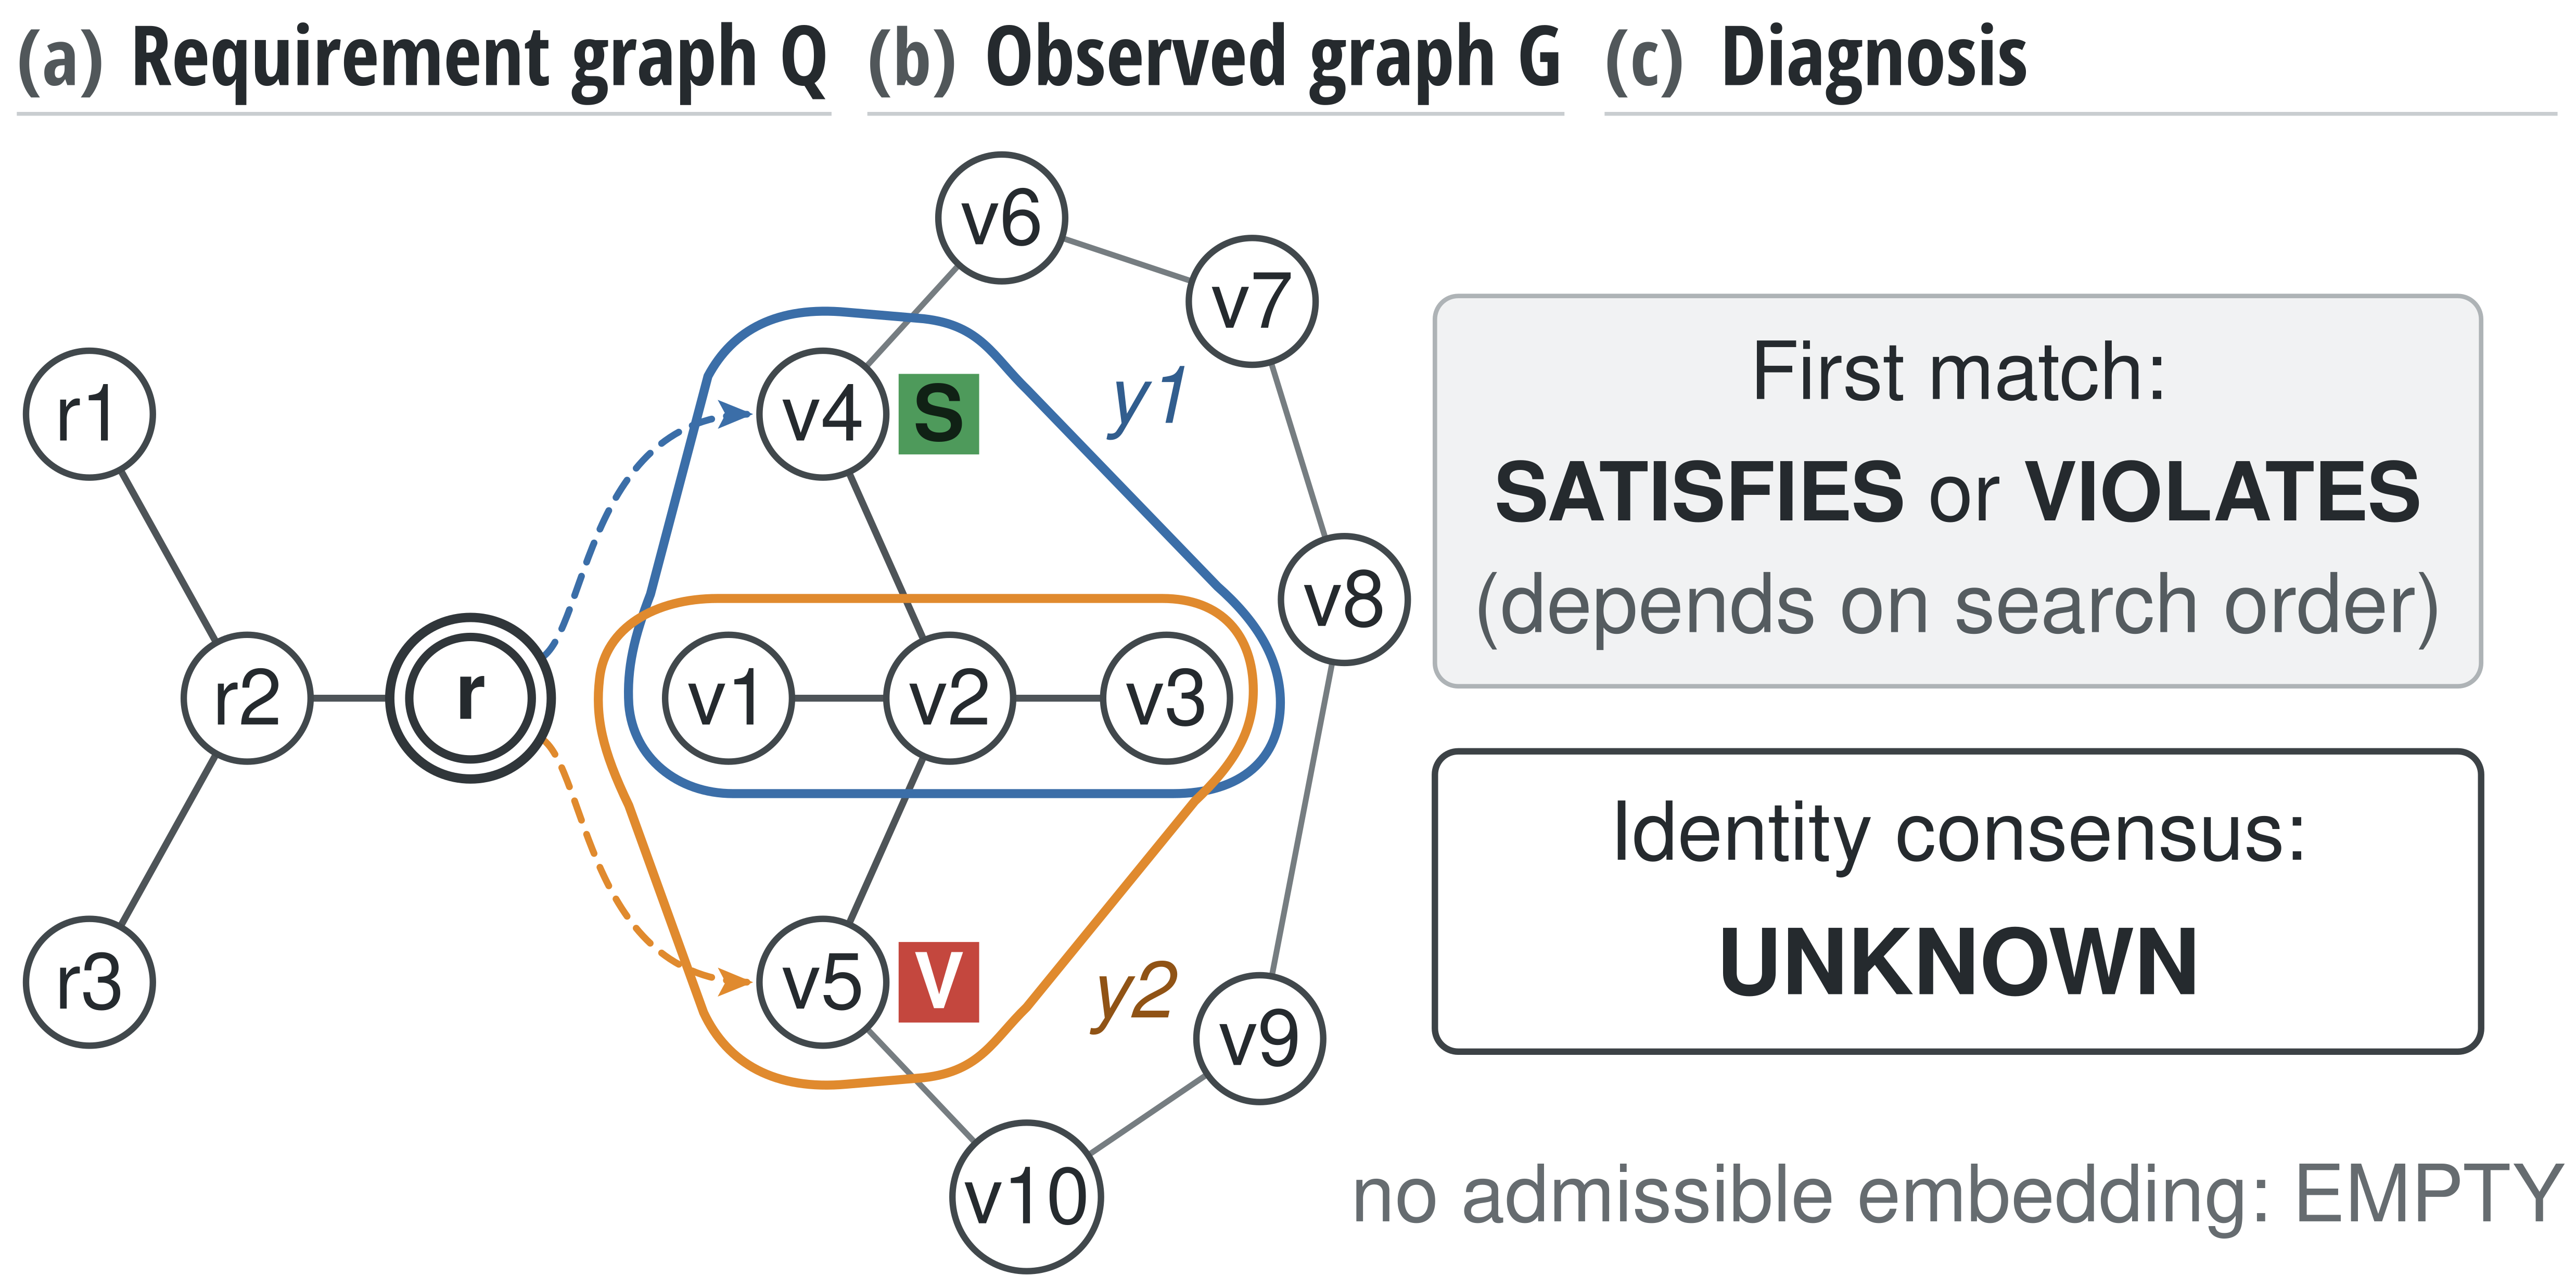
\includegraphics[width=\columnwidth]{figures/fig1_task.png}
\caption{Identity-consensus diagnosis. (a) Requirement graph $Q$ with checked role $r$. (b) Two admissible embeddings $y_1$ (blue) and $y_2$ (orange) in the observed graph $G$ agree on $r_1,r_2,r_3$ but place $r$ on an entity observed as $S$ and on one observed as $V$, respectively. (c) First-match diagnosis reports whichever embedding it finds first; the consensus answer is \Unk{}, and an empty identity space is reported as \Emp{}.}
\label{fig:task}
\end{figure}

\section{Related Work}
\textbf{Subgraph matching.} Exact matching is studied from Ullmann's backtracking \cite{ullmann} through VF2/VF3 \cite{cordella,vf3}, TurboISO \cite{turboiso}, verification-oriented filtering \cite{taming}, failing sets \cite{daf}, compact candidate spaces \cite{bice}, guard-based pruning \cite{gup}, decomposition \cite{asdmatch} and redundant-extension elimination \cite{cemr}; Sun and Luo \cite{sunluo} and RapidMatch \cite{rapidmatch} compare enumeration algorithms on shared query sets. Constraint-based engines such as LAD \cite{lad2010,lad} and the Glasgow Subgraph Solver \cite{glasgow} accept side constraints \cite{side_constraints}, can log proofs \cite{certified,e2everify,auditablecp}, and are combined in portfolios \cite{kotthoff}. Benchmarks for these systems measure the time to find one or all embeddings \cite{sunluo,mccreesh_hard}. IdCon asks a different question of the same engines: an aggregate over all embeddings, which enumeration answers only when the embeddings can be listed.

\textbf{Certain answers and consensus over solutions.} Asking which conclusions hold in every possible world is the certain-answer problem of incomplete databases \cite{imielinski,libkin2011,libkin2014}, studied for graph patterns over incomplete graphs \cite{barcelo}; consistent query answering asks it over the repairs of an inconsistent database \cite{arenas}, with systems that reduce it to integer programming \cite{equip} or SAT \cite{cavsat}, and explainable certain answers attach the witness that blocks a conclusion \cite{certain_answers}. In constraint reasoning the same question is the backbone of a formula \cite{backbones,cadiback} or the cautious consequences of an answer-set program \cite{cautious}, which clingo computes directly \cite{clingo}; IdCon includes both routes as baselines. Our possible worlds are injective, anchored, metric-respecting embeddings, which must be found by subgraph search (NP-hard even for one world \cite{karp,marx}), and the answer has four outcomes, so missing evidence ($U$), violation ($V$) and an empty world set stay distinct. Shape languages for knowledge graphs validate constraints per focus node, with partial assignments when recursion leaves truth values open \cite{shacl}; identity uncertainty in entity resolution is usually handled probabilistically \cite{pasula}, as is uncertain-graph matching with identity linkage \cite{moustafa}, whereas IdCon keeps identities deterministic and asks for consensus; model-based diagnosis \cite{reiter} infers faulty components, whereas IdCon takes observations as given.

\textbf{Benchmark practice.} We follow reproducibility guidance \cite{peng,gundersen,pineau}, document the data with a datasheet \cite{datasheets}, and report completion and penalized runtime as is standard for exact solvers \cite{mccreesh_hard}.

\section{Task}
\label{sec:task}
\textbf{Inputs.} A task consists of a pattern graph $Q=(R,E_Q)$ of roles, an observed graph $G=(N,E_G)$ of entities with coordinates $x:N\to\mathbb{R}^3$, an optional anchor map $a$ fixing some roles to entities, optional metric edges $(r,s,\ell)\in E_Q$ with tolerance $\epsilon$, optional unary domains $D_r\subseteq N$, a set of checked roles $R_c\subseteq R$ with observation tables $p_r:N\to\{S,U,V\}$, and a global state $t_0$, with order $S<U<V$.

\textbf{Identity space.} An admissible identity is an injective map $y:R\to N$ with $y(r)=a(r)$ for anchored roles, $y(r)\in D_r$, $\{y(r),y(s)\}\in E_G$ for every $\{r,s\}\in E_Q$, and $\bigl|\|x_{y(r)}-x_{y(s)}\|-\ell\bigr|<\epsilon$ for every metric edge. Extra observed edges are allowed (non-induced semantics). Let $\mathcal{Y}$ be the set of admissible identities and $T(y)=\max(t_0,\max_{r\in R_c}p_r(y(r)))$ the state of an identity.

\textbf{Outcomes.} The consensus answer is \Emp{} if $\mathcal{Y}=\emptyset$; \Sat{} if $T(y)=S$ for all $y\in\mathcal{Y}$; \Vio{} if $T(y)=V$ for all $y$; and \Unk{} otherwise, i.e., when some identity has state $U$ or the states disagree. A run that stops at its budget without a certified answer returns no answer.

\textbf{Two-query reduction.} Let $\exists(A)$ ask whether some $y\in\mathcal{Y}$ has $T(y)\in A$. Query $\exists(\{S,U,V\})$; a negative answer gives \Emp{}. If the witness has state $U$, the answer is \Unk{}. If it has state $s\in\{S,V\}$, query $\exists(\{S,U,V\}\setminus\{s\})$: a witness gives \Unk{}, a completed negative search gives \Sat{} or \Vio{}. Both queries are existential subgraph problems with unary restrictions: $T(y)\le h$ removes entities with $p_r>h$ from the domain of $r$, and $T(y)\ge l$ is a disjunction over checked roles. Any exact engine that accepts unary domains therefore becomes a consensus solver with at most two calls (or one per checked role for the disjunction), and every positive answer carries a replayable witness. The reduction is standard for certain answers; we state it because it fixes the interface of the IdCon adapters and locates the difficulty in the counterexample query, whose negative answer requires exhausting the search space.

\textbf{Example.} In Figure~\ref{fig:task} the first query may return $y_1$ with state $S$. The counterexample query then restricts $r$ to entities observed $U$ or $V$, finds $y_2$, and the answer is \Unk{}; had it returned $y_2$ first, it would find $y_1$. If $y_2$'s entity were observed $S$, the counterexample query would have to exhaust every identity that places $r$ on a non-$S$ entity before \Sat{} could be reported; a timeout there cannot be read as consensus, which is why IdCon scores unanswered runs separately.

\textbf{Complexity.} Deciding $\mathcal{Y}\neq\emptyset$ generalizes subgraph isomorphism, which contains CLIQUE \cite{karp}, and is NP-complete. \Unk{} is certified by at most two witnesses (an NP certificate); \Emp{} needs a refutation (coNP); \Sat{} and \Vio{} need both a witness and a refutation, so deciding them lies in DP.

\section{The IdCon Benchmark}
\label{sec:bench}
IdCon has five scored suites and two held-out splits (Table~\ref{tab:suites}). The independent unit is a graph-pair \emph{ancestor}: one pattern--host pair; observation tasks that share an ancestor are dependent, and the three HPRD suites share one host. Table~\ref{tab:suites} also reports three priors that predict the label without any search, from the scenario alone, from all metadata, and from a gradient-boosted classifier on metadata and observation-table statistics.

\begin{table*}[t]
\caption{IdCon suites. Labels: assessed references as \Sat/\Vio/\Unk/\Emp. Priors predict the label without search (leave one ancestor out): majority of the scenario, majority of all metadata, and a gradient-boosted classifier on metadata and observation-table statistics. IdCon-HPRD-H and IdCon-Hard-H are held-out splits whose labels are not public; IdCon-Hard-H inputs are also withheld (hashes published). $^\ddagger$: added in stage~3.}
\label{tab:suites}
\centering\footnotesize
\setlength{\tabcolsep}{3.5pt}
\begin{tabular}{lccccccc}
\toprule
 & Hard & Hard-X$^\ddagger$ & HPRD & HPRD-X & Cite$^\ddagger$ & HPRD-H & Hard-H$^\ddagger$\\
\midrule
Source & synthetic & synthetic & \multicolumn{2}{c}{HPRD; third-party queries} & Cora, PubMed & HPRD & synthetic\\
Ancestors / tasks & 72 / 504 & 12 / 72 & 100 / 200 & 96 / 192 & 96 / 192 & 100 / 200 & 12 / 72\\
Entities & 2,048--8,192 & 16,384 & 9,460 & 9,460 & 2,708; 19,717 & 9,460 & 16,384\\
Roles & 48--96 & 128 & 16 & 8--32 & 8--24 & 16 & 128\\
Anchors / metric & 0--2 / yes & 0--2 / yes & no / no & no / no & no / no & no / no & 0--2 / yes\\
Unary domains & no & no & yes & yes & yes & yes & no\\
Assessed refs & 504 & 68 & 200 & 192 & 192 & hidden & hidden\\
Labels & 171/128/161/44 & 21/9/30/8 & 16/99/85/0 & 19/93/80/0 & 14/52/126/0 & hidden & hidden\\
Scenario prior & 339/504 & 45/68 & 183/200 & 170/192 & 134/192 & -- & --\\
Metadata prior & 368/504 & 38/68 & 183/200 & 164/192 & 162/192 & -- & --\\
Learned prior & 419/504 & 52/68 & 181/200 & 166/192 & 162/192 & -- & --\\
\bottomrule
\end{tabular}
\end{table*}


\textbf{IdCon-Hard.} Each ancestor draws a host graph from one of six NetworkX families \cite{networkx} (random geometric, preferential attachment, small-world, random regular, Erd\H{o}s--R\'enyi, articulation modules) at one of three tiers (2,048/48, 4,096/64 or 8,192/96 entities/roles), extracts a pattern by seeded breadth-first search, and keeps either the induced subgraph or its BFS forest. A \emph{plain} variant has no anchors and no metric edges; a \emph{constrained} variant fixes the two highest-degree roles by coordinate and turns 30\% of pattern edges into metric edges on an integer coordinate grid, so that a metric edge prunes candidates without pinning the identity. The full factorial gives 72 ancestors. Eight non-anchored roles are checked. Observation scenarios place labels near the hidden construction embedding $y^*$: \emph{decoys} for a checked role $r$ are entities within one or two hops of $y^*(r)$ that $y^*$ does not use and that have sufficient degree, and a decoy matters exactly when some other admissible embedding maps $r$ there, a property of the graph rather than of the scenario. \textsf{decoy\_v} observes $y^*$ as $S$ and a random fraction of decoys as $V$; \textsf{decoy\_u} uses $U$ for the decoys; \textsf{focal\_v} observes one checked role as $V$ everywhere except at $S$ decoys; \textsf{mixed} combines $U$/$V$ decoys with sparse random violations; \textsf{background} marks a log-uniform fraction of all non-$y^*$ entities $V$; \textsf{perturbed} adds one to three required edges between roles at pattern distance two, which may or may not leave an admissible embedding; and \textsf{decoy\_s}, which turned out to be decided by the observation tables, is a control that the registered analysis keeps in the 504 scored tasks (Section~\ref{sec:prior} reports results without it). No solver is called during generation.

\textbf{IdCon-Hard-X and IdCon-Hard-H.} The same generator at 16,384 entities and 128 roles, with the six families crossed with forest/plain and induced/constrained (12 ancestors) and six scenarios (\textsf{decoy\_s} left out): \hardxTasks{} tasks. IdCon-Hard-H draws \hardhTasks{} tasks the same way with another seed; its inputs and references are not distributed, only their SHA-256 hashes. Its seed is in the released design record, so the split can be regenerated: like IdCon-HPRD-H it is held out by convention, for reporting results on tasks a method was not tuned on, and not a secret test set.

\textbf{IdCon-HPRD, -HPRD-X and -HPRD-H.} All three use the HPRD human protein interaction network as distributed by Sun and Luo \cite{sunluo,hprd} (9,460 entities, 34,998 edges, 307 vertex labels). \emph{IdCon-HPRD} uses the first 100 of their 200 dense 16-vertex query graphs; \emph{IdCon-HPRD-X} adds query graphs of 8, 16, 24 and 32 vertices, dense and sparse, from the public artifact of CEMR \cite{cemr} (12 per set, 96 ancestors); \emph{IdCon-HPRD-H} uses the other 100 Sun--Luo queries with undisclosed references. The benchmark adds two choices only: one to four seeded checked roles per query, and the observation rule. Unchecked roles keep their label as a unary domain; checked roles are free and observe $S$ where the matched entity carries the required label and $V$ otherwise. In \textsf{spec\_true} the required label is the query's own, asking whether the context forces the right protein at the checked positions; in \textsf{spec\_wrong} a different label is drawn by label frequency, modeling a misstated requirement.

\textbf{IdCon-Cite.} Cora (2,708 papers, 7 subject labels) \cite{cora} and PubMed (19,717 papers, 3 labels) \cite{pubmed} as distributed with Planetoid \cite{planetoid}, with their real topology and labels. Queries are extracted in the style of Sun and Luo: a seeded random walk collects $k\in\{8,16,24\}$ vertices and the induced subgraph is a dense (average degree $\ge 3$) or sparse query; 8 per set and host (96 ancestors). The observation rule is that of IdCon-HPRD. Few labels make the label domains wide, so this suite combines real structure with large identity spaces.

\textbf{Format and documentation.} Each task is a JSON identity (coordinates, host edges, role edges with optional lengths, anchors, optional unary domains) plus an observation table; construction maps are stored separately and read only by the reference builder. The release includes manifests with per-ancestor features, SHA-256 hashes of every input, the generators and importers, structural statistics (Appendix Table~\ref{tab:repr}) and a datasheet (Appendix~\ref{app:datasheet}).

\section{Evaluation Protocol}
\label{sec:protocol}
\textbf{References.} References are built by a process that never reads method predictions. For each task and state $s\in\{S,U,V\}$ we decide whether some identity has $T(y)=s$. States excluded by the observation tables are removed directly. The construction map, when admissible, is replayed against all original constraints and settles its own state. Remaining state queries run LAD2025 for 30~s; a LAD negative is re-checked by Glasgow for 30~s and marked \emph{confirmed} when Glasgow also completes; a LAD timeout falls back to Glasgow (60~s) and CP-SAT (60~s). Stage 2 re-queried every unconfirmed negative with Glasgow \texttt{-{}-staged} and CP-SAT and re-settled three IdCon-Hard tasks that stage 1 had settled with one of the authors' solvers (Appendix~\ref{app:registration}). Every positive witness is replayed by a checker. A task is assessed when its label is determined; others are \textsc{Unassessed} and excluded from every denominator. Method witnesses are replayed at scoring time; a replayed witness for a reference negative would invalidate the reference (none did).

\textbf{Independent check.} Because the reference engines are also benchmarked and share the adapters' encoding code, a separate check is written without any benchmark code: it reads the task JSON, encodes each exact-state query $T(y)=s$ in CNF (one-hot roles, at-most-one per entity, support clauses for pattern and metric edges) and solves it with CaDiCaL \cite{cadical}. A witness is replayed against the raw input; a negative is re-derived on the encoding without any pruning and accepted only with a DRAT proof verified by drat-trim \cite{drattrim}. It runs on every IdCon-Hard task with an unconfirmed negative, on 48 stratified random IdCon-Hard tasks, on the IdCon-HPRD-X tasks that ASP-cautious did not answer, on every IdCon-Cite task, and on IdCon-Hard-X on one task per ancestor plus every task with a negative that only one reference engine established. The design record checked every IdCon-Hard-X task with 600\,s per solve; two amendments made during the runs lowered the limits to 120\,s and replaced full coverage of IdCon-Hard-X by this selection, because the check would not have finished on the machine (Appendix~\ref{app:registration}).

\textbf{Methods.} All methods receive the same JSON input and run end to end, including parsing, encoding and process launch, under a 2-second budget on one thread. Two-query adapters (Section~\ref{sec:task}): \emph{LAD} runs LAD2025 \cite{lad} patched to accept unary domains and metric-edge lists; \emph{Glasgow} encodes domains and metric edges as labeled pendant gadgets for the Glasgow Subgraph Solver \cite{glasgow}, whose labelled formats cannot leave some pattern vertices unconstrained; \emph{Glasgow-staged} adds its \texttt{-{}-staged} preprocessing (post hoc on IdCon-Hard and IdCon-HPRD, marked $^\dagger$); \emph{CP-SAT} and \emph{Trad-CP} model identities with AllDifferent and table constraints in OR-Tools. Enumerate-and-aggregate: \emph{Enum-Glasgow} and \emph{Enum-VF2} \cite{networkx,cordella} list identities and stop as soon as two disagree or one has state $U$. Certain-answer reasoning: \emph{ASP-cautious} asks clingo \cite{clingo} for the cautious consequences of $T$; \emph{SAT}$^\ddagger$ runs the two-query reduction on the CNF encoding above with one CaDiCaL process per query. Methods added in stage 2 are marked $^\ast$, those added in stage 3 $^\ddagger$. \emph{First-match} runs one LAD query and reports the state of the first identity.

\textbf{Scoring.} A run is \emph{correct} when its outcome equals the reference. We report correct runs; wrong runs; ancestor-equal PAR-2 (rows averaged within an ancestor, then across ancestors), which charges 4~s for an unanswered or wrong run; and, for uncertified methods, PAR-2 with a 20~s charge per wrong run (PAR-10w). A method that returns a certified outcome contradicting a reference is \emph{unsound} and is not ranked by runtime. The virtual best solver (VBS) takes, per run, any sound method that answers it; we state each time which methods it includes. Strata are compared with ancestor-level bootstrap (10,000 draws), reporting how often a method is best and the interval of its difference to the runner-up; when that interval includes 0 we call the two methods not distinguishable. Each task is run twice per method in a randomized order on a 2-vCPU VM in stages 1 and 2; stage 3 ran on a different 2-vCPU VM that is \calibRatio{} times slower on IdCon-Hard (median ratio over \calibBoth{} runs answered on both machines; \calibAgree{} of \calibRuns{} outcomes agree).

\textbf{Stages and registration.} The study ran in three stages. Stage~1 built IdCon-Hard and IdCon-HPRD and ran LAD, Glasgow, CP-SAT, Trad-CP, first-match and two solvers of the authors; stage~2 added IdCon-HPRD-X, IdCon-HPRD-H, the stage-2 methods and the 10\,s reruns, and dropped the authors' solvers from the benchmark; stage~3 added IdCon-Hard-X, IdCon-Hard-H, IdCon-Cite, SAT, the independent check and the 60\,s reruns. Each stage fixed seeds, factors, methods, budgets, scoring and reference procedure in a hash-stamped design record before its runs; the records and their amendments are released, but their times are the authors' own and not certified by a third party. Several stage-2 and stage-3 analyses were fixed after stage-1 results on the same suites were known; Appendix Table~\ref{tab:registration} says, for every reported analysis, when it was fixed and whether results on the same data were known then.

\section{Results}
\label{sec:results}
\begin{table*}[t]
\caption{Main results under the 2\,s end-to-end budget (two repeats per task). Correct: outcome equals the reference. Wrong: answered but different from the reference; for a certified answer this is a soundness failure (none occurred). PAR-2: ancestor-equal mean, 4\,s for an unanswered or wrong run; best certified method per suite in bold. PAR-10w charges a wrong answer 20\,s instead (it differs from PAR-2 only for uncertified methods). $^\ast$added in stage~2; $^\ddagger$SAT encoding solved by CaDiCaL, added in stage~3; $^\dagger$post hoc arm on Hard and HPRD. Priors predict labels without search, leave one ancestor out, counted per run.}
\label{tab:main}
\centering\small\setlength{\tabcolsep}{4.5pt}
\begin{tabular}{l rrr rrr rrr}
\toprule
 & \multicolumn{3}{c}{IdCon-Hard (1,008 runs)} & \multicolumn{3}{c}{IdCon-HPRD (400 runs)} & \multicolumn{3}{c}{IdCon-HPRD-X (384 runs)}\\
\cmidrule(lr){2-4}\cmidrule(lr){5-7}\cmidrule(lr){8-10}
Method & Correct & Wrong & PAR-2 & Correct & Wrong & PAR-2 & Correct & Wrong & PAR-2\\
\midrule
LAD & 725 & 0 & \textbf{1,635} & 389 & 0 & 1,036 & 199 & 0 & 2,513\\
Glasgow & 562 & 0 & 2,113 & 0 & 0 & 4,000 & 1 & 0 & 3,995\\
Glasgow-staged$^\dagger$ & 651 & 0 & 1,740 & 304 & 0 & 1,361 & 265 & 0 & 1,734\\
CP-SAT & 321 & 0 & 2,998 & 384 & 0 & 455 & 360 & 0 & 830\\
Trad-CP & 214 & 0 & 3,347 & 279 & 0 & 1,858 & 191 & 0 & 2,603\\
Enum-Glasgow$^\ast$ & 88 & 0 & 3,688 & 235 & 0 & 2,638 & 65 & 0 & 3,568\\
Enum-VF2$^\ast$ & 14 & 0 & 3,951 & 127 & 0 & 2,937 & 74 & 0 & 3,354\\
ASP-cautious$^\ast$ & 15 & 0 & 3,968 & 400 & 0 & 748 & 365 & 0 & 1,230\\
SAT$^\ddagger$ & 240 & 0 & 3,378 & 400 & 0 & \textbf{374} & 384 & 0 & \textbf{380}\\
\midrule
First-match (PAR-2 / PAR-10w) & 626 & 315 & 1,901 / 6,901 & 230 & 170 & 2,027 / 8,827 & 224 & 160 & 2,242 / 8,909\\
Metadata prior & 736 & 272 & -- & 366 & 34 & -- & 328 & 56 & --\\
Learned prior & 838 & 170 & -- & 362 & 38 & -- & 332 & 52 & --\\
\bottomrule
\end{tabular}
\end{table*}


\subsection{Embeddings are rarely unique; first-match is wrong where they disagree}
\label{sec:firstmatch}
What carries over to other workloads is how often embeddings are not unique, which does not depend on our observation rule. Counting embeddings with Glasgow (30~s per query), \hprdCountFullMulti{} of the \hprdCountFullQueries{} IdCon-HPRD queries have more than one embedding when every query vertex must match its own label, and \hprdAutoOrbitMulti{} still do after dividing by the number of label-preserving automorphisms of the query, i.e., counting genuinely different placements (\hprdCountFullThousand{} queries have at least 1,000 embeddings; no count hit the time limit); on IdCon-HPRD-X the figures are \hprdxCountFullMulti{} and \hprdxAutoOrbitMulti{} of \hprdxCountFullQueries{}. With the checked roles freed, \hprdCountSpaceMulti{} and \hprdxCountSpaceMulti{} of the identity spaces have more than one identity.

A first match can be wrong only on an \Unk{} task: if the reference is \Sat{} or \Vio{} every identity has that state, and if it is \Emp{} there is nothing to report. Every wrong first-match run in IdCon is indeed on an \Unk{} task (\hardFirstWrongOnUnknown{} of \hardFirstWrong{} on IdCon-Hard, \hprdFirstWrongOnUnknown{} of \hprdFirstWrong{} on IdCon-HPRD, \hprdxFirstWrongOnUnknown{} of \hprdxFirstWrong{} on IdCon-HPRD-X; Table~\ref{tab:main}). Its error rate on a suite is therefore the share of tasks whose embeddings disagree, a property of the workload rather than a finding: \hardFirstWrongAnsweredPct\% of answered IdCon-Hard runs, set by the generator's decoy rates, and \hprdFirstWrongPct\% of IdCon-HPRD runs, set by the observation rule (\hprdFirstWrongSpecTrue{} of the \hprdFirstWrong{} wrong runs are \textsf{spec\_true} tasks).

\subsection{Exact methods are sound, and none dominates}
\label{sec:exact}
No exact method returned a certified outcome that contradicts a reference on any suite, and all \witnessTotalRtwo{} positive witnesses returned by methods on the five scored suites replay against the original constraints. On IdCon-Hard, \hardBest{} has the lowest PAR-2 (\hardBestPar~ms; runner-up \hardSecond{}, \hardSecondPar~ms). On IdCon-HPRD and IdCon-HPRD-X, \hprdBest{} and \hprdxBest{} have (\hprdBestPar{} and \hprdxBestPar~ms; runners-up \hprdSecond{} and \hprdxSecond{}, \hprdSecondPar{} and \hprdxSecondPar~ms), and \hprdMost{} and \hprdxMost{} answer the most runs (\hprdMostCorrect{} of \hprdASPcautiousAssessed{} and \hprdxMostCorrect{} of \hprdxASPcautiousAssessed{}). The SAT baseline thus leads where label domains are narrow, yet answers only \hardSATCorrect{} of \hardSATAssessed{} IdCon-Hard runs, where its encoding grows with the number of candidates per role. Inside the suites the best method changes with size, anchoring and query size (Appendix Figure~\ref{fig:strata} and Tables~\ref{tab:strata-hard}--\ref{tab:strata-hprdx}); with the share of bootstrap resamples in which it stays best in brackets, and n.s.\ where it is not distinguishable from the runner-up, \strataSentence{}. With 12 ancestors per IdCon-Hard stratum these comparisons are coarse. At 2\,s the best single method leaves \hardBestUnsolvedPct\% of IdCon-Hard runs unsolved; a VBS over the methods registered in stages 1 and 2 (Glasgow-staged excluded as a post hoc arm) leaves \hardVBSUnsolved{} runs (\hardVBSUnsolvedPct\%), and one over every sound method including Glasgow-staged and SAT leaves \hardVBSAllUnsolved{} (\hardVBSAllUnsolvedPct\%). These figures describe the benchmarked methods at 2\,s, not a limit of exact methods: two unpublished solvers of the authors, run in stage~1 and not part of the benchmark, answer \legEgCorrect{} and \legSvCorrect{} of the 1,008 IdCon-Hard runs at 2\,s, and with them the VBS leaves \legVBSBoth{} (Appendix Table~\ref{tab:legacy}).

\begin{table}[t]
\caption{Stage-3 suites (repeat~0, one run per task and budget on IdCon-Hard-X; two repeats at 2\,s on IdCon-Cite). Correct runs within 2, 10 and 60\,s (a run unanswered at a budget is rerun at the next for the methods listed in the design record; -- not rerun). VBS: tasks that no sound method answers within the budget. No certified answer contradicts a reference.}
\label{tab:newsuites}
\centering\footnotesize
\setlength{\tabcolsep}{2.6pt}
\begin{tabular}{lrrr rrr}
\toprule
 & \multicolumn{3}{c}{IdCon-Hard-X (68 tasks)} & \multicolumn{3}{c}{IdCon-Cite (192 tasks)}\\
\cmidrule(lr){2-4}\cmidrule(lr){5-7}
Method & 2\,s & 10\,s & 60\,s & 2\,s$^{2}$ & PAR-2 & 10\,s\\
\midrule
LAD & 1 & 30 & 64 & 192 & 2,086 & 191\\
Glasgow & 1 & 29 & -- & 92 & 3,256 & --\\
Glasgow-staged & 15 & 33 & 46 & 126 & 2,904 & 107\\
CP-SAT & 5 & 11 & -- & 124 & 2,911 & 88\\
Trad-CP & -- & -- & -- & 190 & 2,188 & --\\
Enum-Glasgow$^\ast$ & 1 & 4 & -- & 104 & 3,118 & --\\
Enum-VF2$^\ast$ & -- & -- & -- & 77 & 3,300 & --\\
ASP-cautious$^\ast$ & -- & -- & -- & 223 & 1,964 & 192\\
SAT$^\ddagger$ & 2 & 2 & 40 & 265 & 1,598 & 192\\
\midrule
First-match & 1 & 35 & -- & 114 & 2,837 & --\\
\midrule
VBS unsolved & 49 & 23 & 3 & 110 & -- & 0\\
\bottomrule
\end{tabular}
\end{table}


\subsection{Larger hosts and real labels}
\label{sec:newsuites}
The stage-3 suites change the picture where IdCon-Hard is near saturation (Table~\ref{tab:newsuites}). On IdCon-Hard-X, where one LAD2025 query alone takes about 3\,s on a 16,384-entity host, the methods jointly leave \hardxVBSUnsolvedTwo{} of \hardxComplete{} assessed tasks unanswered at 2\,s, \hardxVBSUnsolvedTen{} at 10\,s and \hardxVBSUnsolvedSixty{} at 60\,s; the best single method answers \hardxBestSingleTenN{} within 10\,s (\hardxBestSingleTen{}) and \hardxBestSingleSixtyN{} within 60\,s (\hardxBestSingleSixty{}). Glasgow-staged answers most at 2\,s, LAD after its slow first query. On IdCon-Cite, whose few labels leave wide domains on real citation graphs, the fastest sound method is \citeBest{} (PAR-2 \citeBestPar~ms), the certain-answer formulations (ASP-cautious, SAT) are competitive with the two-query adapters, and the methods jointly leave \citeVBSUnsolvedRuns{} of the 2\,s runs unanswered and \citeVBSUnsolvedTen{} tasks at 10\,s. No certified answer contradicts a reference on either suite.

\begin{figure*}[t]
\centering
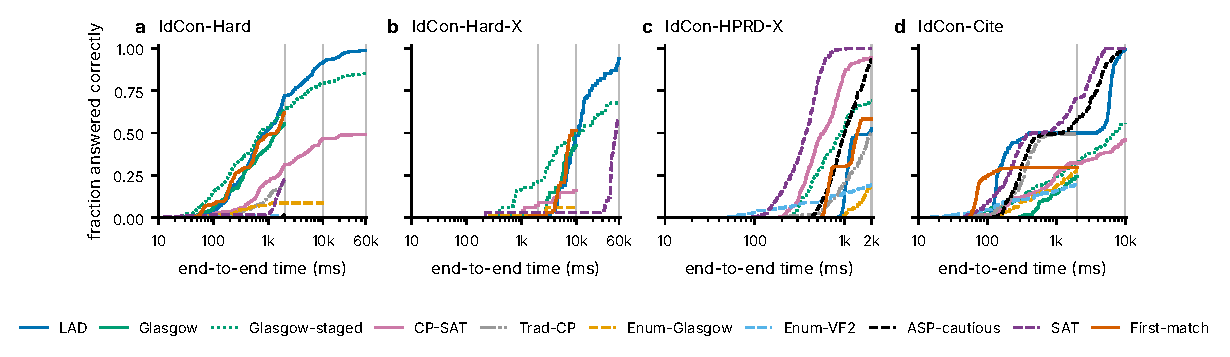
\includegraphics[width=\textwidth]{figures/fig2_results.pdf}
\caption{Fraction of assessed tasks answered correctly within a given end-to-end time (repeat~0). Runs unanswered at 2\,s continue with the 10\,s rerun and, for the methods rerun at 60\,s, with the 60\,s rerun (grey lines: 2, 10 and 60\,s). (a) IdCon-Hard, (b) IdCon-Hard-X, (c) IdCon-HPRD-X, (d) IdCon-Cite. Dashed: methods added in stages 2 and 3. Times after the first budget on IdCon-Hard come from the stage-3 machine (\calibRatio{} times slower).}
\label{fig:results}
\end{figure*}

\subsection{Budget, overhead and headroom}
\label{sec:budget}
The difficulty of IdCon-Hard is largely a 2\,s difficulty (Figure~\ref{fig:results}a). On repeat~0, LAD answers \hardLadRepTwo{} of 504 tasks at 2\,s, \hardLadRepTen{} at 10\,s and \hardLadRepSixty{} at 60\,s; the VBS over every sound method leaves \hardVBSAllUnsolvedTwo{}, \hardVBSAllUnsolvedTen{} and \hardVBSAllUnsolvedSixty{} tasks unanswered (at 60\,s: \hardVBSSixtyLabels{}). IdCon-Hard therefore separates methods at short budgets and is close to solved with a minute per task; IdCon-Hard-X separates them at 10\,s (Section~\ref{sec:newsuites}). On IdCon-HPRD every method rerun at 10\,s reaches at least \hprdGlasgowTenS{} of \hprdRepZeroN{} tasks, and ASP-cautious and SAT answer \hprdASPcautiousCorrect{} and \hprdSATCorrect{} of its \hprdSATAssessed{} runs at 2\,s; that suite's 2\,s ranking measures per-call start-up cost more than search. The cost is visible directly. On IdCon-HPRD one LAD call on a one-role pattern takes \ovhLadOneRole~ms end to end and one default Glasgow call \ovhGlasgowOneRole~ms. On 48 stratified IdCon-Hard tasks, the first LAD query takes \ovhHardLadTotal~ms (median), of which \ovhHardLadOutside~ms are spent outside the solver process (building the graph, writing files) and the solver process \ovhHardLadSolver~ms; for Glasgow-staged the figures are \ovhHardGSTotal, \ovhHardGSOutside{} and \ovhHardGSSolver~ms. Results at one budget should be read with the completion curves, and adapter engineering is part of what the 2\,s budget measures.

\subsection{Tools and universal outcomes}
\label{sec:tools}
On IdCon-Hard, where by degree almost every entity is a candidate for every role, enumeration and grounding do not finish: Enum-Glasgow answers \hardEnumGlasgowCorrect{}, Enum-VF2 \hardEnumVFTwoCorrect{} and ASP-cautious \hardASPcautiousCorrect{} of \hardEnumGlasgowAssessed{} runs. Where label domains are narrow (HPRD) the certain-answer formulations are the most complete methods: ASP-cautious and SAT answer \hprdxASPcautiousCorrect{} and \hprdxSATCorrect{} of the \hprdxSATAssessed{} IdCon-HPRD-X runs. \Unk{} needs witnesses only, whereas \Sat{}, \Vio{} and \Emp{} need a completed negative search, and the methods differ most on the latter: on IdCon-Hard, LAD answers \hardLADSatCorrect{} \Sat{} runs and CP-SAT \hardCPSATSatCorrect{}, against \hardLADUnkCorrect{} and \hardCPSATUnkCorrect{} \Unk{} runs (Appendix Table~\ref{tab:labels}).

\subsection{What can be predicted without search}
\label{sec:prior}
On IdCon-Hard the scenario alone predicts \hardPriorScenario{} references, all metadata \hardPriorMeta{}, and the learned prior \hardPriorLearned{} (\hardPriorLearnedPct\%); \priorWrongAllThree{} references defeat all three priors. Two shortcuts explain much of this. First, in \sensDecided{} tasks (\sensDecidedPct\%; \sensDecidedDecoyS{} of them the \textsf{decoy\_s} control) the observation tables exclude two of the three states in a scenario whose construction embedding is admissible, so one existence query decides the label; a method that adds this table check gains these runs. Second, on the HPRD suites the scenario fixes the label for \hprdPriorScenario{} and \hprdxPriorScenario{} tasks, because a misstated label is rarely carried by an admissible embedding. The ranking of the exact methods is robust to both: without \textsf{decoy\_s} and without all \sensDecided{} table-decided tasks, \sensRankSentence{} (post hoc, Appendix Table~\ref{tab:sensitivity}). On IdCon-Hard-X and IdCon-Cite the learned prior reaches \hardxPriorLearned{} and \citePriorLearned{}. A learned predictor has to beat these numbers before its accuracy reflects the graph; for exact methods the shortcuts only mean that part of a suite is easy. Because the released tools compute exact labels from public inputs (IdCon-HPRD-H) or from a public seed (IdCon-Hard-H), the held-out splits guard against tuning, not against a determined user.

\begin{table}[t]
\caption{Independent reference check: an encoding written without any benchmark code, solved by CaDiCaL; witnesses replayed against the raw input; negatives decided on the unpruned encoding with DRAT proofs verified by drat-trim. Settles: tasks \textsc{Unassessed} in the reference that the check decides. Limits: 600\,s per solve and 1,200\,s per proof check (registered) for the first 4 tasks, 120\,s and 300\,s for the rest (Amendment~6); Hard-X single-engine negatives: every IdCon-Hard-X task with a negative state that only one reference engine established, not already sampled (Amendment~7).}
\label{tab:idcheck}
\centering\footnotesize
\setlength{\tabcolsep}{3pt}
\begin{tabular}{lrrrrr}
\toprule
Sample & Tasks & Agree & Disagree & Unresolved & Settles\\
\midrule
Hard, unconfirmed negative & 17 & 10 & 0 & 7 & 0\\
Hard, stratified random & 48 & 44 & 0 & 4 & 0\\
HPRD-X, no ASP answer & 4 & 4 & 0 & 0 & 0\\
Cite, all tasks & 192 & 192 & 0 & 0 & 0\\
Hard-X, one per ancestor & 12 & 10 & 0 & 1 & 1\\
Hard-X, single-engine negative & 19 & 19 & 0 & 0 & 0\\
\midrule
Total & 292 & 279 & 0 & 12 & 1\\
\bottomrule
\end{tabular}
\end{table}


\subsection{Reference quality}
\label{sec:refquality}
Every positive state is a replayed witness. Of the \hardNegRone{} non-trivial IdCon-Hard negatives, \hardNegRoneCorroborated{} are confirmed by a second engine after the stage-2 re-check (\hardNegVoneCorroborated{} of \hardNegVone{} after stage~1); on IdCon-HPRD all \hprdNegRone{} are, and on IdCon-HPRD-X \hprdxNegRoneCorroborated{} of \hprdxNegRone{}. The second engines are themselves benchmarked and share the adapters' code, so we added the independent check of Section~\ref{sec:protocol} (Table~\ref{tab:idcheck}): it decides \idcDecided{} of \idcTasks{} sampled and new-suite tasks, agrees with \idcAgree{} references, contradicts \idcDisagree{} and decides \idcSettles{} that the reference procedure left \textsc{Unassessed} (\idcUnresolved{} unresolved; \idcDrat{} negative states carry verified DRAT proofs), including \idcUnconfAgree{} of the \idcUnconfTasks{} IdCon-Hard tasks whose negatives no second engine had confirmed. The new suites need it most on IdCon-Hard-X, where Glasgow corroborates only \hardxNegCorroborated{} of \hardxNeg{} non-trivial negatives within its 30\,s on the 16,384-entity hosts (IdCon-Cite: \citeNegCorroborated{} of \citeNeg{}); the check agrees on \idcHardxSingleAgree{} of the \idcHardxSingleTasks{} IdCon-Hard-X tasks with such a single-engine negative (\idcHardxSingleUnresolved{} unresolved) and on \idcCiteAgree{} of \idcCiteTasks{} IdCon-Cite tasks. Restricted to fully confirmed references, the ranking of the sound methods \refRankSentence{} (Appendix Table~\ref{tab:refs}).


\section{Using IdCon}
\textbf{Interface.} A method receives the identity record, the observation tables and a budget, and returns an outcome, a certificate flag and every positive witness it found. The driver measures the full call; nothing in it gives a method access to construction maps or references. Adding a method needs one adapter function and one dispatch line.

\textbf{What to report.} Per suite: correct, wrong and unanswered runs; ancestor-equal PAR-2; correct runs by reference label (Appendix Table~\ref{tab:labels}), because a method that only finds witnesses looks strong on \Unk{} and weak elsewhere; completion curves to at least 60\,s; and the number of certified outcomes that disagree with the reference, which must be zero for an exact method. Approximate and learned methods leave the certificate flag unset and must beat the learned prior of Table~\ref{tab:suites}. Predictions on the held-out splits are scored by the maintainers.

\textbf{Extending IdCon.} The generator exposes its factors (family, tier, density, construction, anchors, metric fraction, scenario parameters) and is deterministic given a seed; harder tiers can be added without touching existing records, as IdCon-Hard-X shows. A new population should be registered before it is run and should report its no-search priors.

\section{Reproducibility and Release}
The release contains, per suite, the generator or importer, input hashes, protected construction maps, references with their engine logs, frozen predictions, the independent checker, scoring code and a read-only verifier that recomputes every table and number of this paper from the frozen records. Adapters, the patched LAD2025 sources (CeCILL-B) and build scripts are included; Glasgow, CaDiCaL, drat-trim, clingo, NetworkX and OR-Tools are obtained upstream with versions and hashes recorded. Project code is MIT and our generated data, references and predictions are CC BY 4.0, at \url{\repourl}. HPRD is free for academic, non-commercial use only, the CEMR query files carry no licence, and Cora and PubMed are taken from the MIT-licensed Planetoid repository; none is redistributed: scripts fetch them from pinned upstream commits and check their hashes, and task files built from them are generated locally. Rebuilt binaries reproduce labels, not timings.

\section{Limitations and Ethics}
\label{sec:limits}
The synthetic suites are not samples of engineering requirement graphs; the HPRD and Cite suites supply real topology and labels with our checked-role choice and observation rule, so observations are label agreement rather than measured defects. No suite comes from a deployed requirement-checking system. Negative references are solver-trusted except where the independent check verified a DRAT proof; we report confirmation rates and results restricted to confirmed references. Methods that launch external processes pay that cost per query, in-process methods do not, and the 2\,s budget measures that cost as well as search (Section~\ref{sec:budget}); budgets are enforced by killing solver processes and by time checks in Python-side encoding, so an encoding phase can overrun (scored as unanswered). Timings come from two 2-vCPU VMs with two concurrent single-thread processes; the two repeats agree on \hardRepeatAgreePct\% (Hard), \hprdRepeatAgreePct\% (HPRD) and \hprdxRepeatAgreePct\% (HPRD-X) of outcomes, the last because many HPRD-X runs finish close to the budget. The two solvers run in stage~1 and then left out of the benchmark are the authors' own unpublished methods; their results are disclosed (Appendix Table~\ref{tab:legacy}) but not ranked.

The benchmark contains no personal data. A consensus checker can make an engineering or biological check stricter; it cannot certify that the requirement graph itself is right, and \Sat{} should not be read as validation of the requirement.

\section{Discussion}
\textbf{For practitioners.} The shortcut is safe only when the admissible embedding is unique, and on the third-party queries it rarely is (Section~\ref{sec:firstmatch}). A cheap safeguard follows from the reduction: after a first match, issue the counterexample query. If it completes without a witness, the first-match answer was right; if it finds one, the answer is \Unk{}; if it times out, report the result as undetermined rather than as the first-match label.

\textbf{For solver designers.} The suites reward different engines: LAD's propagation on large unanchored ambiguous patterns, Glasgow's staged preprocessing on the largest hosts, and SAT and cautious reasoning when label domains are narrow or the identity space is small enough to ground; whole-model CP wins some anchored strata. IdCon-Hard is a short-budget suite: with a minute per task the benchmarked methods jointly leave \hardVBSAllUnsolvedSixty{} of its 504 tasks open, and unpublished methods already do better at 2\,s (Appendix Table~\ref{tab:legacy}). IdCon-Hard-X moves the separating budget up: within 10\,s the best single method answers \hardxBestSingleTenN{} of its \hardxComplete{} assessed tasks and all methods together leave \hardxVBSUnsolvedTen{} open, while \hardxBestSingleSixty{} answers \hardxBestSingleSixtyN{} with 60\,s. IdCon-Cite is a 2\,s suite: some method answers every task within 10\,s, but at 2\,s the best single method answers \citeBestSingleTwoN{} of \citeTasks{}. None of the suites is beyond exact search with a minute per task, so IdCon measures the cost of exact consensus rather than its feasibility; the released generator scales further. The hardest outcomes are the universal ones, where proving \Sat{} requires refuting every non-$S$ placement; the independent check shows that DRAT proofs for such refutations are practical for many IdCon instances, so proof-producing consensus solvers \cite{auditablecp} can be held to certified negatives.


\section{Conclusion}
IdCon makes identity-consensus diagnosis measurable. Admissible embeddings are rarely unique in third-party query workloads, even up to query symmetry, so a match-then-read check is wrong wherever they disagree; how often that happens is a property of the workload. Exact consensus is sound with every engine we tried, and no engine dominates: two-query adapters, whole-model CP, enumeration, cautious reasoning and SAT each win somewhere and fail somewhere else. How hard the benchmark is depends on the budget and the suite: IdCon-Hard and IdCon-Cite separate methods at 2\,s, IdCon-Hard-X at 10\,s, and with a minute per task the methods together answer nearly every task, so what IdCon measures is the cost of exact consensus. The benchmark fixes the interface, references with an independent proof-checked sample, scoring, and two held-out splits, so that new consensus engines, including proof-producing and learned ones, can be compared directly.

